\documentclass{standalone}
\usepackage[x11names]{xcolor}
\usepackage{tikz}
\begin{document}
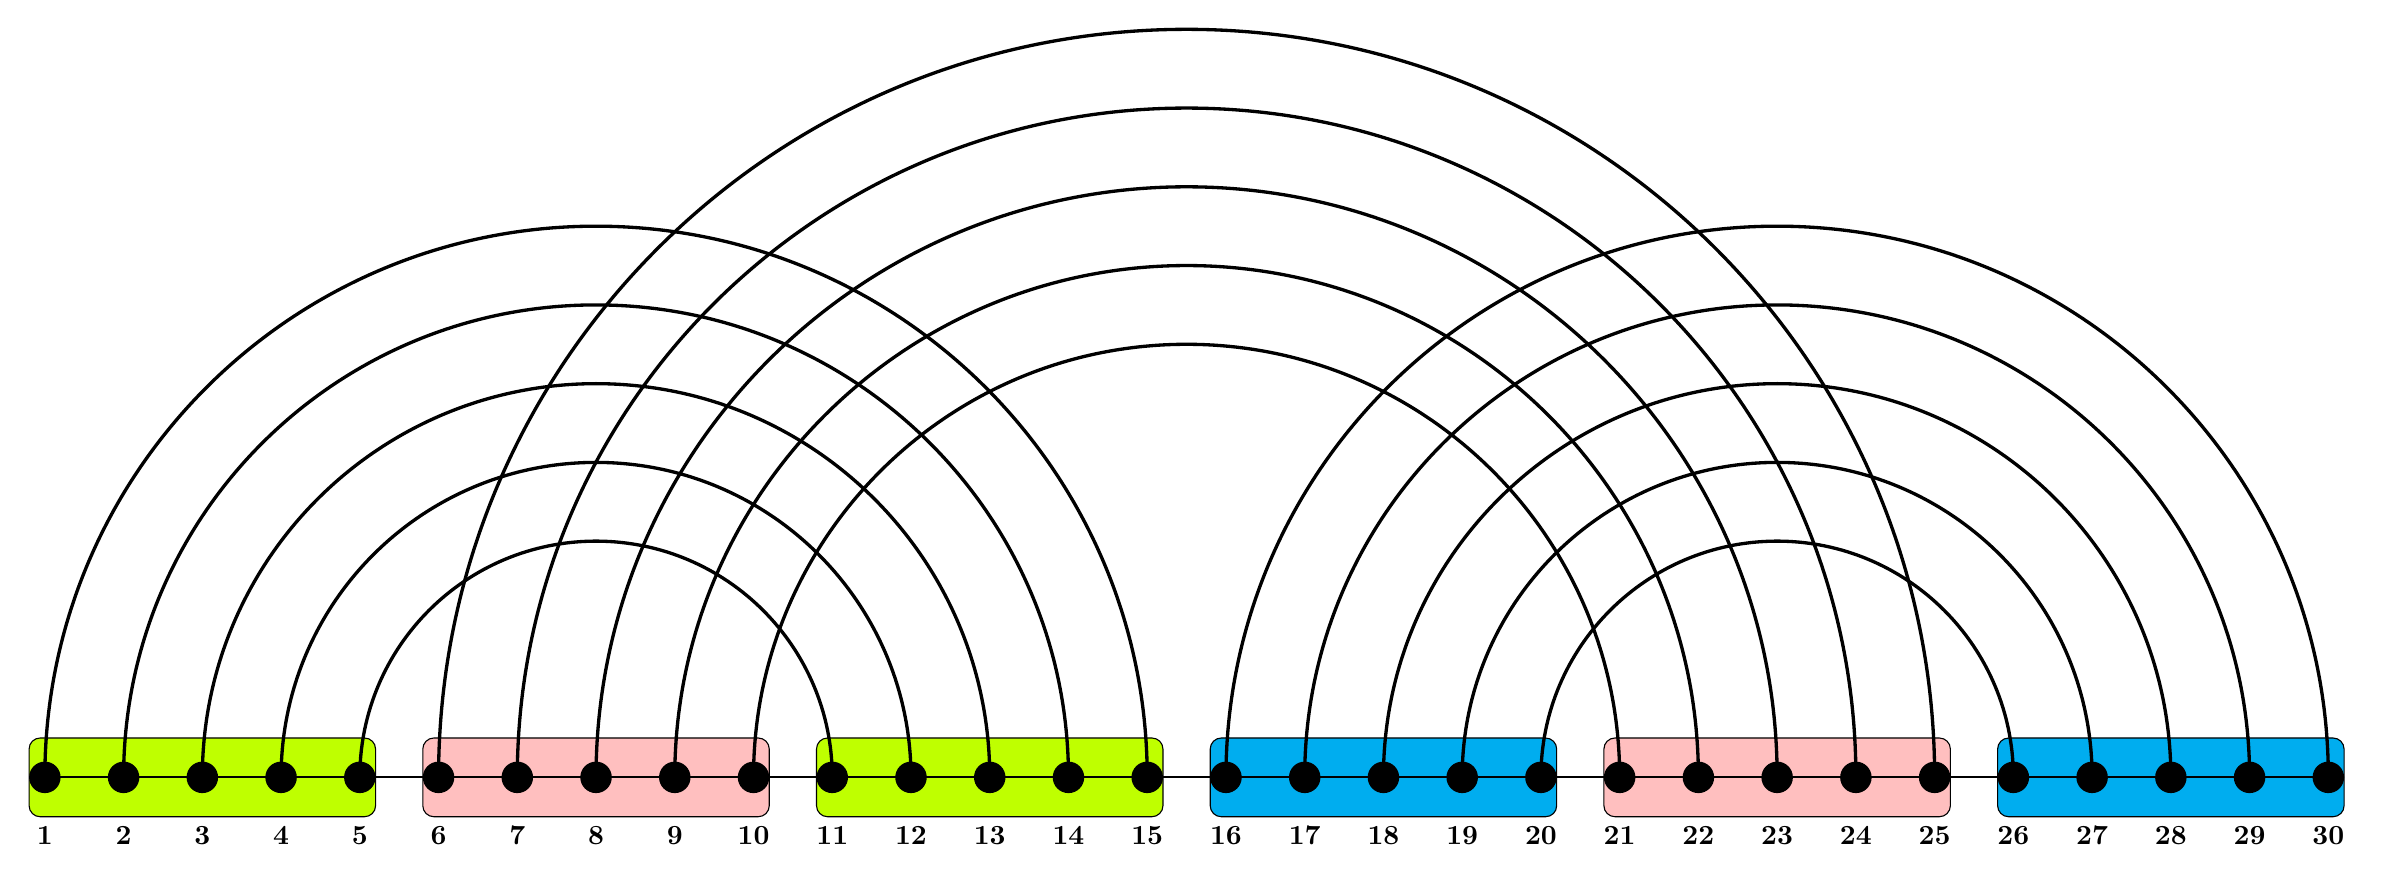
\begin{tikzpicture}
\filldraw[fill=lime,rounded corners]  (-0.2,-0.5) rectangle (4.2,+0.5);
\filldraw[fill=lime,rounded corners]  (9.8,-0.5) rectangle (14.2,+0.5);
\filldraw[fill=pink,rounded corners]  (4.8,-0.5) rectangle (9.2,+0.5);
\filldraw[fill=pink,rounded corners]  (19.8,-0.5) rectangle (24.2,+0.5);
\filldraw[fill=cyan,rounded corners]  (14.8,-0.5) rectangle (19.2,+0.5);
\filldraw[fill=cyan,rounded corners]  (24.8,-0.5) rectangle (29.2,+0.5);
\fill (0,0) circle (0.2) node[below=.5cm] {\textbf{1}};
\fill (1,0) circle (0.2) node[below=.5cm] {\textbf{2}};
\fill (2,0) circle (0.2) node[below=.5cm] {\textbf{3}};
\fill (3,0) circle (0.2) node[below=.5cm] {\textbf{4}};
\fill (4,0) circle (0.2) node[below=.5cm] {\textbf{5}};
\fill (5,0) circle (0.2) node[below=.5cm] {\textbf{6}};
\fill (6,0) circle (0.2) node[below=.5cm] {\textbf{7}};
\fill (7,0) circle (0.2) node[below=.5cm] {\textbf{8}};
\fill (8,0) circle (0.2) node[below=.5cm] {\textbf{9}};
\fill (9,0) circle (0.2) node[below=.5cm] {\textbf{10}};
\fill (10,0) circle (0.2) node[below=.5cm] {\textbf{11}};
\fill (11,0) circle (0.2) node[below=.5cm] {\textbf{12}};
\fill (12,0) circle (0.2) node[below=.5cm] {\textbf{13}};
\fill (13,0) circle (0.2) node[below=.5cm] {\textbf{14}};
\fill (14,0) circle (0.2) node[below=.5cm] {\textbf{15}};
\fill (15,0) circle (0.2) node[below=.5cm] {\textbf{16}};
\fill (16,0) circle (0.2) node[below=.5cm] {\textbf{17}};
\fill (17,0) circle (0.2) node[below=.5cm] {\textbf{18}};
\fill (18,0) circle (0.2) node[below=.5cm] {\textbf{19}};
\fill (19,0) circle (0.2) node[below=.5cm] {\textbf{20}};
\fill (20,0) circle (0.2) node[below=.5cm] {\textbf{21}};
\fill (21,0) circle (0.2) node[below=.5cm] {\textbf{22}};
\fill (22,0) circle (0.2) node[below=.5cm] {\textbf{23}};
\fill (23,0) circle (0.2) node[below=.5cm] {\textbf{24}};
\fill (24,0) circle (0.2) node[below=.5cm] {\textbf{25}};
\fill (25,0) circle (0.2) node[below=.5cm] {\textbf{26}};
\fill (26,0) circle (0.2) node[below=.5cm] {\textbf{27}};
\fill (27,0) circle (0.2) node[below=.5cm] {\textbf{28}};
\fill (28,0) circle (0.2) node[below=.5cm] {\textbf{29}};
\fill (29,0) circle (0.2) node[below=.5cm] {\textbf{30}};
\draw[thick] (0,0) -- (1,0);
\draw[thick] (1,0) -- (2,0);
\draw[thick] (2,0) -- (3,0);
\draw[thick] (3,0) -- (4,0);
\draw[thick] (4,0) -- (5,0);
\draw[thick] (5,0) -- (6,0);
\draw[thick] (6,0) -- (7,0);
\draw[thick] (7,0) -- (8,0);
\draw[thick] (8,0) -- (9,0);
\draw[thick] (9,0) -- (10,0);
\draw[thick] (10,0) -- (11,0);
\draw[thick] (11,0) -- (12,0);
\draw[thick] (12,0) -- (13,0);
\draw[thick] (13,0) -- (14,0);
\draw[thick] (14,0) -- (15,0);
\draw[thick] (15,0) -- (16,0);
\draw[thick] (16,0) -- (17,0);
\draw[thick] (17,0) -- (18,0);
\draw[thick] (18,0) -- (19,0);
\draw[thick] (19,0) -- (20,0);
\draw[thick] (20,0) -- (21,0);
\draw[thick] (21,0) -- (22,0);
\draw[thick] (22,0) -- (23,0);
\draw[thick] (23,0) -- (24,0);
\draw[thick] (24,0) -- (25,0);
\draw[thick] (25,0) -- (26,0);
\draw[thick] (26,0) -- (27,0);
\draw[thick] (27,0) -- (28,0);
\draw[thick] (28,0) -- (29,0);
\draw[very thick] (11,0) arc                 (0:180:4.0);
\draw[very thick] (25,0) arc                 (0:180:3.0);
\draw[very thick] (12,0) arc                 (0:180:5.0);
\draw[very thick] (13,0) arc                 (0:180:6.0);
\draw[very thick] (20,0) arc                 (0:180:5.5);
\draw[very thick] (26,0) arc                 (0:180:4.0);
\draw[very thick] (14,0) arc                 (0:180:7.0);
\draw[very thick] (27,0) arc                 (0:180:5.0);
\draw[very thick] (22,0) arc                 (0:180:7.5);
\draw[very thick] (21,0) arc                 (0:180:6.5);
\draw[very thick] (28,0) arc                 (0:180:6.0);
\draw[very thick] (29,0) arc                 (0:180:7.0);
\draw[very thick] (24,0) arc                 (0:180:9.5);
\draw[very thick] (23,0) arc                 (0:180:8.5);
\draw[very thick] (10,0) arc                 (0:180:3.0);
\end{tikzpicture}
\end{document}
